\section{Auswertung}
\label{sec:Auswertung}

% % Examples
% \begin{equation}
%   U(t) = a \sin(b t + c) + d
% \end{equation}
%
% \begin{align}
%   a &= \input{build/a.tex} \\
%   b &= \input{build/b.tex} \\
%   c &= \input{build/c.tex} \\
%   d &= \input{build/d.tex} .
% \end{align}
% Die Messdaten und das Ergebnis des Fits sind in Abbildung~\ref{fig:plot} geplottet.
%
% %Tabelle mit Messdaten
% \begin{table}
%   \centering
%   \caption{Messdaten.}
%   \label{tab:data}
%   \sisetup{parse-numbers=false}
%   \begin{tabular}{
% % format 1.3 bedeutet eine Stelle vorm Komma, 3 danach
%     S[table-format=1.3]
%     S[table-format=-1.2]
%     @{${}\pm{}$}
%     S[table-format=1.2]
%     @{\hspace*{3em}\hspace*{\tabcolsep}}
%     S[table-format=1.3]
%     S[table-format=-1.2]
%     @{${}\pm{}$}
%     S[table-format=1.2]
%   }
%     \toprule
%     {$t \:/\: \si{\milli\second}$} & \multicolumn{2}{c}{$U \:/\: \si{\kilo\volt}$\hspace*{3em}} &
%     {$t \:/\: \si{\milli\second}$} & \multicolumn{2}{c}{$U \:/\: \si{\kilo\volt}$} \\
%     \midrule
%     \input{build/table.tex}
%     \bottomrule
%   \end{tabular}
% \end{table}
%
% % Standard Plot
% \begin{figure}
%   \centering
%   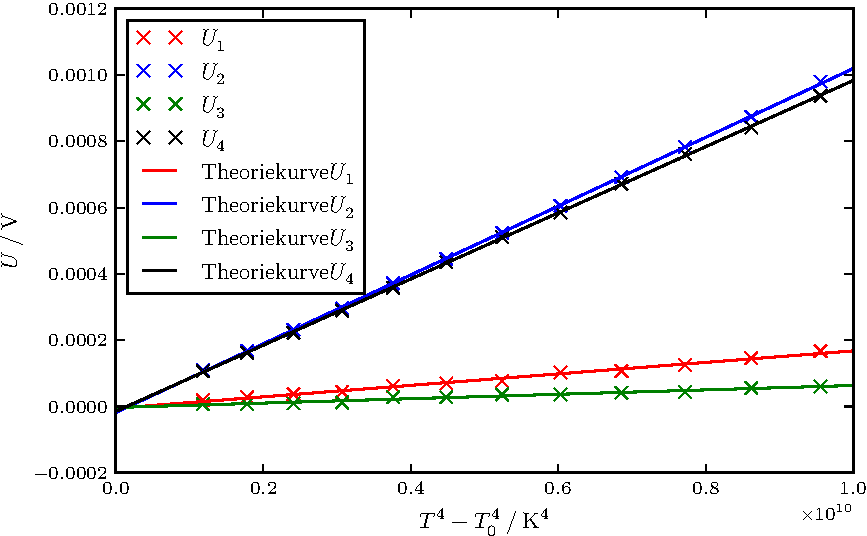
\includegraphics{build/plot.pdf}
%   \caption{Messdaten und Fitergebnis.}
%   \label{fig:plot}
% \end{figure}
%
% 2x2 Plot
% \begin{figure*}
%     \centering
%     \begin{subfigure}[b]{0.475\textwidth}
%         \centering
%         \includegraphics[width=\textwidth]{Abbildungen/Schaltung1.pdf}
%         \caption[]%
%         {{\small Schaltung 1.}}
%         \label{fig:Schaltung1}
%     \end{subfigure}
%     \hfill
%     \begin{subfigure}[b]{0.475\textwidth}
%         \centering
%         \includegraphics[width=\textwidth]{Abbildungen/Schaltung2.pdf}
%         \caption[]%
%         {{\small Schaltung 2.}}
%         \label{fig:Schaltung2}
%     \end{subfigure}
%     \vskip\baselineskip
%     \begin{subfigure}[b]{0.475\textwidth}
%         \centering
%         \includegraphics[width=\textwidth]{Abbildungen/Schaltung4.pdf}    % Zahlen vertauscht ... -.-
%         \caption[]%
%         {{\small Schaltung 3.}}
%         \label{fig:Schaltung3}
%     \end{subfigure}
%     \quad
%     \begin{subfigure}[b]{0.475\textwidth}
%         \centering
%         \includegraphics[width=\textwidth]{Abbildungen/Schaltung3.pdf}
%         \caption[]%
%         {{\small Schaltung 4.}}
%         \label{fig:Schaltung4}
%     \end{subfigure}
%     \caption[]
%     {Ersatzschaltbilder der verschiedenen Teilaufgaben.}
%     \label{fig:Schaltungen}
% \end{figure*}

\subsection{Überprüfung der Bragg Bedingung}
Um die ausreichende Kalibrierung des Gerätes festzustellen, wird zunächst die in der Durchführung beschriebene Kontrolle der Bragg-Bedingung durchgeführt.
Die Ergebnisse der Messung sind in Abbildung \ref{fig:plot1} dargestellt.
\begin{figure}
  \centering
  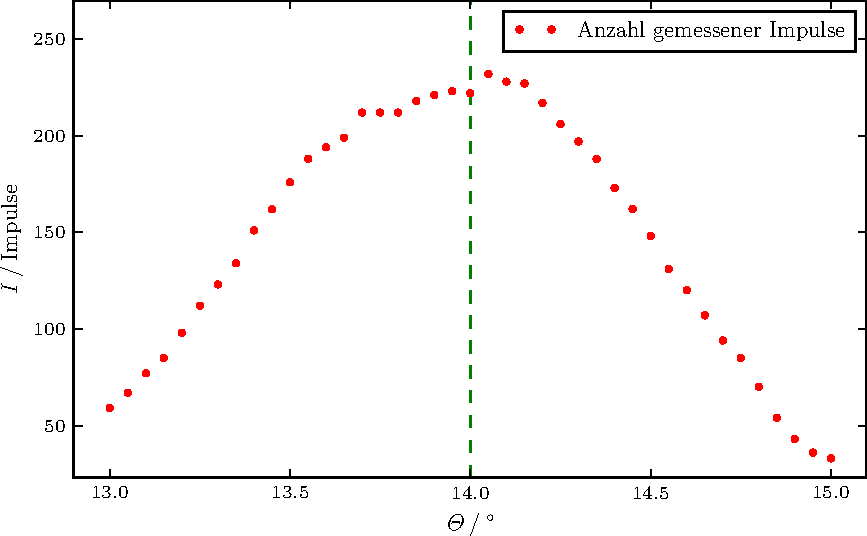
\includegraphics{build/plot_1.pdf}
  \caption{Messwerte zur Prüfung der Bragg Bedingung.}
  \label{fig:plot1}
\end{figure}
Der Peak ist in etwa gleichmäßig um den erwarteten Winkel von $\Theta = \SI{14}{\degree}$ zentriert.

\subsection{Emissionsspektrum der Kupfer-Röntgen-Röhre}
\subsubsection{Analyse der Peaks und Grenzwellenlänge}
Wie in der Durchführung beschrieben wird das Emissionsspektrum der Röntgenröhre durchlaufen.
Das gemessene Röntgenspektrum ist in Abbildung \ref{fig:plot2} angegeben.
\begin{figure}
  \centering
  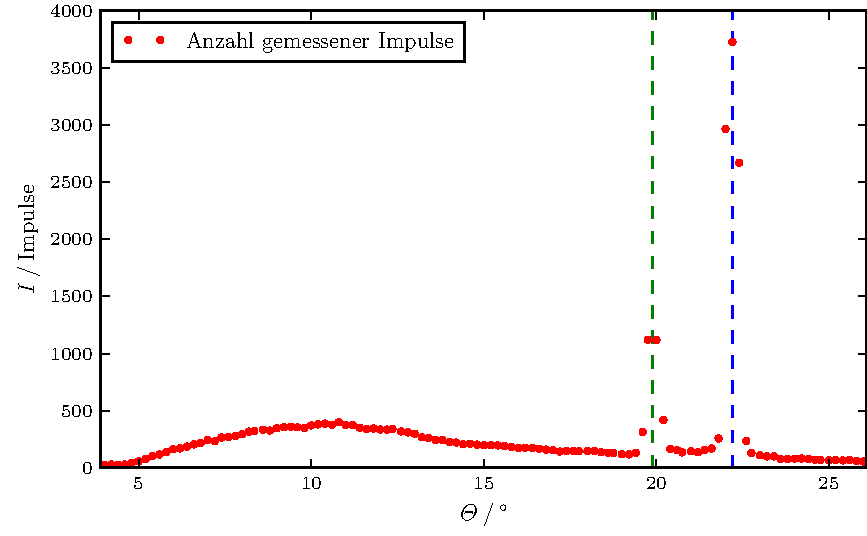
\includegraphics{build/plot_2.pdf}
  \caption{Emissionsspektrum der Kupfer-Anode.}
  \label{fig:plot2}
\end{figure}
Als Peaks des Spektrums lassen sich die Winkel
\begin{align*}
   \Theta_{K_\alpha} &= \SI{22.2}{\degree}
  \\
   \Theta_{K_\beta} &= \SI{19.9}{\degree}
 \\
\end{align*}
ablesen und als die jeweiligen Linien identifizieren.
Nach Formel \eqref{eqn:bragg} bestimmen sich die dazugehörigen Energien zu
\begin{align*}
  E_{K_\alpha} &= \SI{8.15}{\kilo\electronvolt}
 & E_{K_\alpha, \text{lit}} &= \SI{8.0}{\kilo\electronvolt}
 \\
  E_{K_\beta} &= \SI{9.05}{\kilo\electronvolt}
 & E_{K_\beta, \text{lit}} &= \SI{8.9}{\kilo\electronvolt}
 .
\end{align*}
Zudem sind jeweils die dazugehörigen Literaturwerte \cite{energie} angegeben.\\
Zur Untersuchung des Bremsbergs bzw. zur Bestimmung der maximalen Energie des Bremsspektrums wird das Emissionsspektrum für den Grenzbereich ein weiteres mal mit einer höheren Auflösung gemessen.
Das Ergebnis ist in Abbildung \ref{fig:plot3} graphisch dargestellt.
\begin{figure}
  \centering
  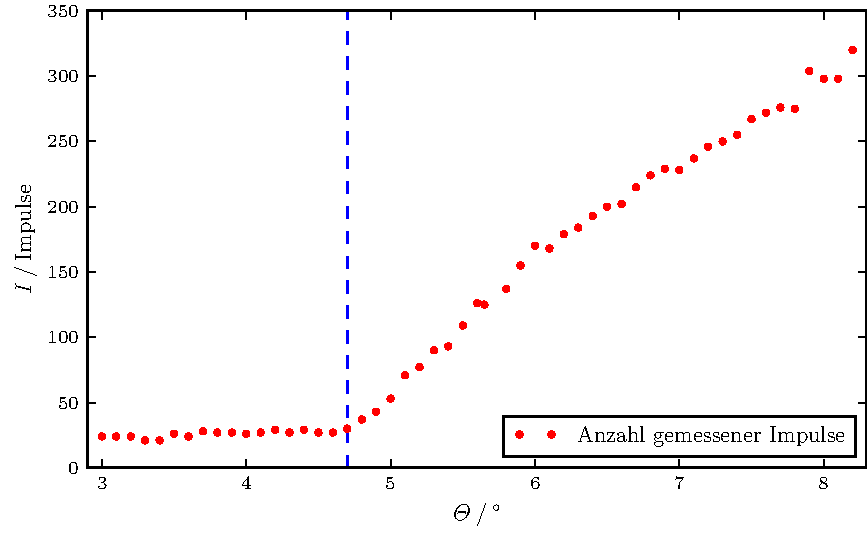
\includegraphics{build/plot_3.pdf}
  \caption{Emissionsspektrum der Kupfer-Anode (Maximale Kante).}
  \label{fig:plot3}
\end{figure}
Der auftretende Grenzwinkel beträgt
\begin{align*}
  \Theta_{\text{grenz}} = \SI{4.7}{\degree}
 \\
\end{align*}
was sich mit Hilfe von Formel \eqref{eqn:bragg} zu einer minimalen Wellenlänge von
\begin{align*}
  \lambda_{\text{min}} = \SI{33.0}{\pico\metre}

\end{align*}
beziehungsweise einer maximalen Energie von
\begin{align*}
  E_{\text{max}} = \SI{37.6}{\kilo\electronvolt}

\end{align*}
umrechnen lässt.
Aufgrund der genutzten Beschleunigungsspannung von $U_\text{B} = \SI{35}{\volt}$ wird nach Formel \eqref{eqn:l} eine theoretische minimale Wellenlänge von
\begin{align*}
  \lambda_{\text{min,t}} = \SI{35.4}{\pico\metre}

\end{align*}
beziehungsweise eine maximalen Energie von
\begin{align*}
  E_{\text{max,t}} = \SI{35.0}{\kilo\electronvolt}

\end{align*}
erwartet.
\subsubsection{Bestimmung der Abschirmkonstanten für Kupfer}
Aus den Energien $E_{K_\alpha}$ und $E_{K_\beta}$ lassen sich aus Formel \eqref{eqn:std} die Abschirmkonstanten $\sigma_K$ bestimmen.
Für $\sigma_1$ wird verwendet, dass die Absorptionskante hier in etwa mit der Bindungsenergie des Elektrons übereinstimmt.
Die Abschirmkonstante wird somit nach Formel \eqref{eqn:std} ermittelt.
Für $\sigma_2$ wird die Abschirmkonstante aus der Beziehung $E_{k_\alpha} = E_2 - E_1$, für $sigma_3$ aus der Beziehung  $E_{k_\beta} = E_3 - E_1$ gewonnen.
Es ergeben sich somit die Abschirmkonstanten
\begin{align*}
  \sigma_{1} &= \SI{3.2}{ }
 & \sigma_{1, \text{lit}} &= \SI{3.41}{ }
 \\
  \sigma_{2} &= \SI{12.7}{ }
 & \sigma_{2, \text{lit}} &= \SI{13.12}{ }
 \\
  \sigma_{3} &= \SI{27.39}{ }
 & \sigma_{3, \text{lit}} &= \SI{21.96}{ }

\end{align*}
sowie im Vergleich dazu die dazugehörigen Literaturwerte, welche mithilfe der Literaturwerte \cite{energie} für die Energien errechnet werden.

\subsubsection{Bestimmung der Halbwertsbreite}
Zur Bestimmung der Halbwertsbreite werden die Messwerte an den jeweligen Peaks genauer betrachtet.

\begin{table}
  \hspace*{\fill}
  \begin{subfigure}{0.40\textwidth}
  \centering
  %\caption{Messdaten Teil 1.}
  \label{tab:2a}
  \sisetup{table-format=3.4}
  \begin{tabular}{c c}
    \toprule
     {$\Theta \:/\: \si{\degree}$} & {$I \:/\: \text{Impulse}$}\\
    \midrule
    19.4  & 131 \\
19.6  & 313 \\
19.8  & 1120  \\
20.0  & 1118  \\
20.2  & 419 \\
20.4  & 165 \\
20.6  & 154 \\

    \bottomrule
  \end{tabular}
\end{subfigure}
\hspace*{\fill}
\begin{subfigure}{0.40\textwidth}
  \centering
  %\caption{Messdaten Teil 2.}
  \label{tab:2b}
  \sisetup{table-format=3.4}
  \begin{tabular}{c c}
    \toprule
     {$\Theta \:/\: \si{\degree}$} & {$I \:/\: \text{Impulse}$}\\
    \midrule
    21.6  & 169 \\
21.8  & 257 \\
22.0  & 2966  \\
22.2  & 3729  \\
22.4  & 2671  \\
22.6  & 324 \\
22.8  & 130 \\

    \bottomrule
  \end{tabular}
\end{subfigure}
\\
\hspace*{\fill}
\hspace*{\fill}
\caption{Messdaten zur Frequenzabhängigen Amplituden und Phasenverschiebungsbestimmung.}
\label{tab:2}
\end{table}
Aufgrund der zu geringen Auflösung der Messung wird das Verhalten des Graphen zwischen dem Anfang und der Mitte des Peaks sowie der Mitte und dem Ende des Peaks jeweils als linear angenommen.
Anhand dieser linearen Näherung werden die Winkel bestimmt, an denen die Hälfte des Peaks erreicht wird und die dazugehörige Energie bestimmt.
Es ergeben sich hieraus für den ersten Peak Auflösungswerte von
\begin{align*}
  \increment \Theta_1 &= \SI{0.50}{\degree}
 \\
  \increment E_1 &= \SI{0.22}{\kilo\electronvolt}
 \\
\end{align*}
und für den zweiten Peak Auflösungswerte von
\begin{align*}
  \increment \Theta_2 &= \SI{0.60}{\degree}
 \\
  \increment E_2 &= \SI{0.21}{\kilo\electronvolt}
. \\
\end{align*}

\subsection{Analyse der Absorbtionsspektren}
Für die Elemente Germanium ($Z=32$), Zirkonium ($Z=40$) und Strontium ($Z=38$) werden wie in der Durchführung angegeben die Absorbtionsspektren aufgenommen.
In den Abbildungen \ref{fig:plot4}, \ref{fig:plot5} und \ref{fig:plot6} sind die Messungen jeweils graphisch dargestellt, wobei in blau die Linie eingezeichnet wird, an der die K-Kante abgelesen wird.

\begin{figure}
  \centering
  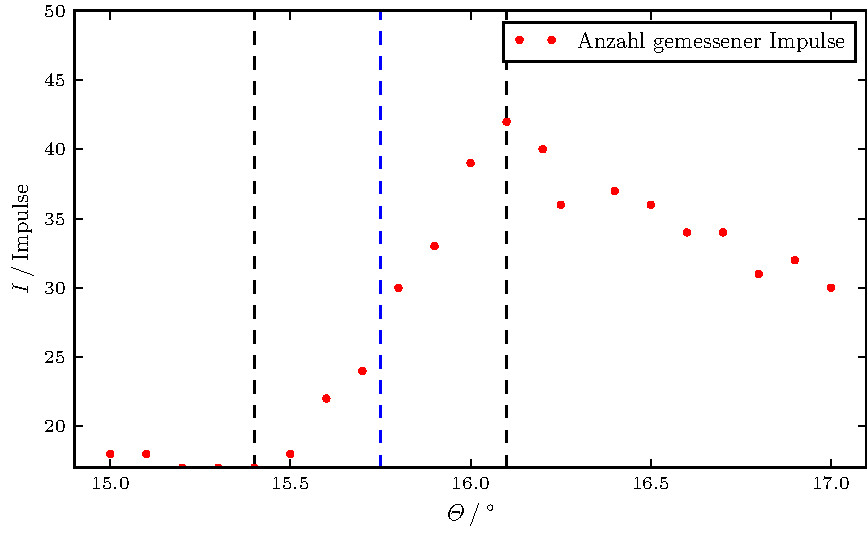
\includegraphics{build/plot_ge.pdf}
  \caption{Absorbtionsspektrum von Germanium (K-Kante).}
  \label{fig:plot4}
\end{figure}

\begin{figure}
  \centering
  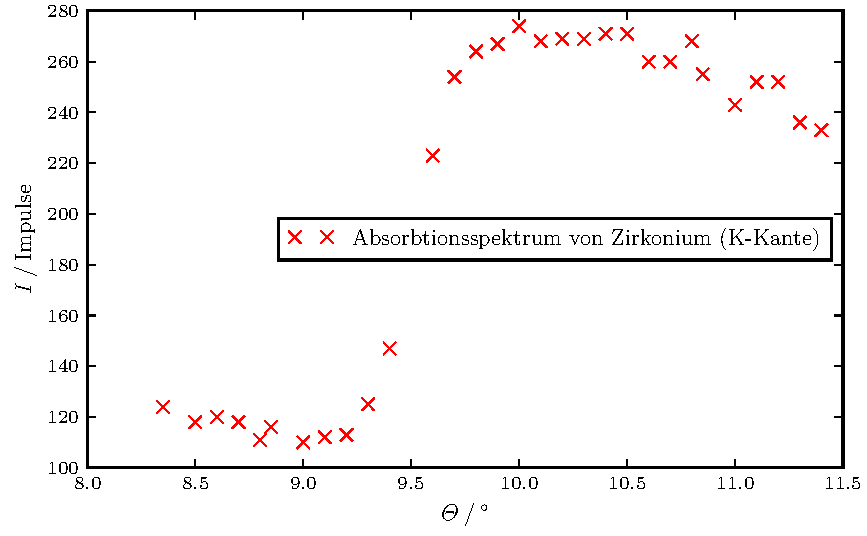
\includegraphics{build/plot_zr.pdf}
  \caption{Absorbtionsspektrum von Zirkonium (K-Kante).}
  \label{fig:plot5}
\end{figure}

\begin{figure}
  \centering
  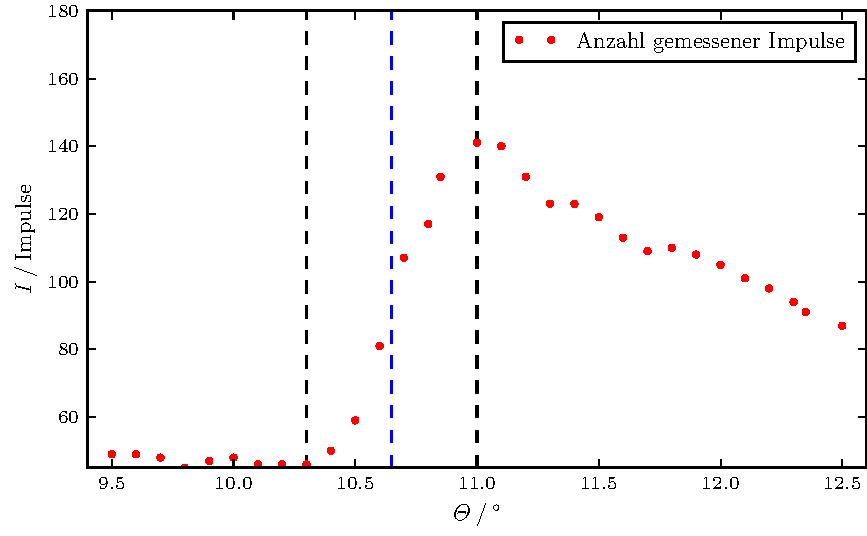
\includegraphics{build/plot_sr.pdf}
  \caption{Absorbtionsspektrum von Strontium (K-Kante).}
  \label{fig:plot6}
\end{figure}

Anhand von Formel \eqref{eqn:l} ergeben sich für die Energieübergänge die Werte
\begin{align*}
  E_\text{Ge} &= \SI{11.34}{\kilo\electronvolt}
, \\
  E_\text{Zr} &= \SI{18.46}{\kilo\electronvolt}
, \\
  E_\text{Sr} &= \SI{16.66}{\kilo\electronvolt}
. \\
\end{align*}
Hieraus ergeben sich nach Formel \eqref{eqn:std} die Abschirmzahlen
\begin{align*}
  \sigma_\text{Ge} &= \SI{3.13}{ }
, \\
  \sigma_\text{Zr} &= \SI{3.17}{ }
, \\
  \sigma_\text{Sr} &= \SI{0.88}{ }
. \\
\end{align*}
Die Literaturwerte, welche anhand der Energien der K-Kante aus der Literatur \cite{energie} berechnet werden, sind
\begin{align*}
  \sigma_\text{Ge, lit} &= \SI{3.43}{ }
, \\
  \sigma_\text{Zr, lit} &= \SI{38.78}{ }
, \\
  \sigma_\text{Sr, lit} &= \SI{3.60}{ }
. \\
\end{align*}

\subsection{Bestimmung der Rydbergkonstante aus dem Moseleyschen Gesetz}
Die Rydbergkonstante kann mithilfe des Moseleyschen Gesetzes \eqref{eqn:std} bestimmt werden.
Hierzu wird der Wert von $Z_\text{eff}$ gegen die Wurzel der dazugehörigen Energie des $K_\alpha$ Übergangs abgetragen.
Diese Werte werden mithilfe von Numpy in Python linear gefittet. Das Ergebnis ist in Abbildung \ref{fig:plot7} dargestellt.
\begin{figure}
  \centering
  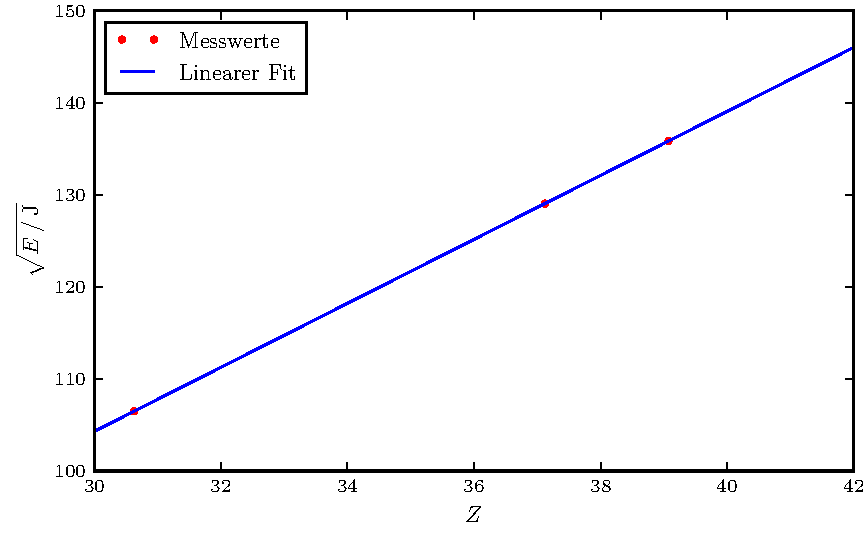
\includegraphics{build/plot_ryd.pdf}
  \caption{Bestimmung der Rydbergkonstante.}
  \label{fig:plot7}
\end{figure}
Hieraus kann zunächst auf die Rydbergenergie von
\begin{align*}
  R_y &= \SI{18.14092013+-0.00000002}{\electronvolt}
, \\
\end{align*}
und darauf unverzüglich auf die Rydbergkonstante von
\begin{align*}
  R_{\infty} &= \SI{13000461.7+-0.3}{\per\metre}
, \\
\end{align*}
geschlossen werden.

\subsection{Bestimmung der Abschirmkonstante von Wismut}
Für das Element Wismut lässt sich die Abschirmkonstante aufgrund der höheren Kernladungszahl nach Formel \eqref{eqn:crap} bestimmen.
Hierzu wird das Absorbtionsspektrum im Bereich der L-Kanten betrachtet. Das Ergebnis ist in Abbildung \ref{fig:plot8} dargestellt.
\begin{figure}
  \centering
  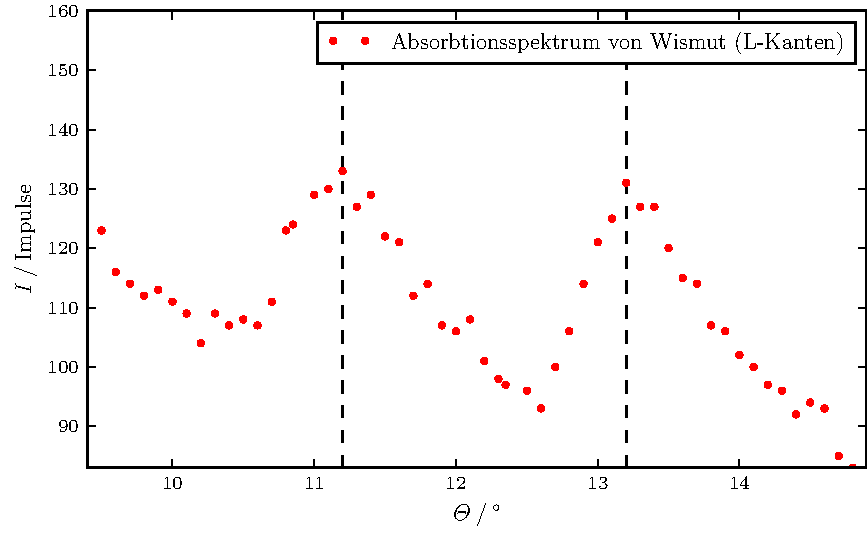
\includegraphics{build/plot_wi.pdf}
  \caption{Absorbtionsspektrum von Wismut.}
  \label{fig:plot8}
\end{figure}
Aus dem Spektrum kann man die Kanten für die Winkel
\begin{align*}
  \Theta_{\text{Bi},1} &= \SI{10.9}{\degree}
, \\
  \Theta_{\text{Bi},2} &= \SI{13.2}{\degree}
 \\
\end{align*}
entnehmen.
Hieraus folgt eine Energiedifferenz von
\begin{align*}
  \increment E_\text{L} &= \SI{2367.6}{\electronvolt}
. \\
\end{align*}
Aus der Formel \eqref{eqn:crap} folgt hiermit für die Abschirmkonstante von Wismut
\begin{align*}
  \sigma_{\text{Bi}} &= \SI{3.03}{ }
, \\
  \sigma_\text{Bi, lit} &= \SI{3.61}{ }
,
\end{align*}
wobei der Literaturwert ebenfalls anhand von Formel \eqref{eqn:crap} aus den bekannten Literaturenergien \cite{energie} berechnet wird.
